\documentclass[../../../main.tex]{subfiles}
\begin{document}
Il peut être intéressant de stocker des éléments selon un ordre et de vouloir très rapidement trouver le minimum ou le maximum de ces éléments selon l'ordre choisi. Quelques exemples sont donnés pour montrer l'intérêt d'une structure spécialisé pour cette opération. 

\textbf{Exemple (\textit{context-switching}) :} dans un système d'exploitation, les tâches sont exécutés en alternance pour simuler leur exécution parallèle. On veut sélectionner des tâches 
\begin{itemize}
	\item qui depuis longtemps n'ont pas été traités
	\item qui sont demandantes en ressources
\end{itemize}
On peut associer à chaque tâche une pondération de chaque critère qui correspond à sa \textit{priorité}. On veut alors à chaque changement de tâche sélectionner celle de plus haute priorité. Comme le changement de tâche en lui-même doit consommer très peu de ressources, on veut une structure de données efficace, donc spécialisé pour ce but.

\textbf{Exemple (algorithmes gloutons) :} de nombreux algorithmes cherchent à optimiser numériquement des solutions en cherchant d'abord un optimum local dans l'espace des solutions. Si les différents choix sont organisés selon une file de priorité, la sélection de l'optimum local est très rapide et accélère grandement l'algorithme. C'est ce qu'on retrouve dans l'algorithme de \textit{Dijkstra} pour la recherche d'un plus court chemin dans un graphe.
\subsection{Signature}
\textbf{Première remarque :} il suffit de définir une structure de donnée permettant de trouver rapidement le minimum des élémeents. En effet, il suffit juste d'inverser la relation d'ordre pour obtenir une structure permettant de trouver rapidement le maximum des éléments.

\textit{Element} désigne un type de donnée sur lequel est défini une relation d'ordre totale\footnote{Partielle suffit en soi d'après le théorème de Szpilrajn.}

\textit{FilePriorite\textless{}Element\textgreater} utilise \textit{Booleen}, \textit{Element}
\begin{itemize}
	\item $file\_vide()\rightarrow FilePriorite$ renvoie une file de priorité sans éléments
	\item $est\_vide(f:FilePriorite)\rightarrow Booleen$ teste si la file $f$ est vide.
	\item $minimum(f:FilePriorite)\rightarrow Element$ renvoie l'élément minimal de la file de priorité
	\item $supprimer\_min(f:FilePriorite)\rightarrow FilePriorite$ renvoie $f$ dont on a retiré l'élément minimal
	\item $inserer(f:FilePriorite:f, x:Element)\rightarrow FilePriorite$ renvoie $f$ à laquelle on a ajouté $x$
\end{itemize}
On construit la routine de commodité $extraire\_min(\text{mut }FilePriorite:f)\rightarrow Element$ qui renvoie l'élément minimal de $f$ et le supprime de $f$.

On implanter les files de priorité par des arbres AVLs. Les complexités temporelles des routines $minimum$ $supprimer\_min$ et $inserer$ sont alors des fonctions de $O(log_2(n))$, où $n$ est le nombre d'éléments dans la file de priorité.

On présente ici une autre implantation plus efficace et bien plus simple à mettre en oeuvre, le \textit{tas minimum}.
\subsection{Arbres complets}
Les tas minimums forment un cas particulier d'arbres presque complets. On définit donc d'abord cette notion et comment on peut implanter très facilement et très efficacement des arbres presque complets.
\subsubsection{Principe}
\definition{Arbres presque complets} {
	L'ensemble $A^p_X$ des \textit{arbres presque complets} sur un ensemble ordonné $(X, \leq)$ est défini par induction par :
	$$\left\{\begin{array}{cll}
	\mathcal{B} & : & E\in A^p_X \\
	\mathcal{I} & : & \forall g, d\in A^p_X, \forall x\in X, (0 \leq h(g) - h(d) \leq 1) \Rightarrow (g, x, d)\in A^p_X
\end{array}\right.$$
	En français : pour tout sous-arbre $(g, x, d)$ d'un arbre,
	\begin{itemize}
		\item le sous-arbre gauche est toujours plus haut que le sous-arbre droit
		\item le sous-arbre est équilibré
	\end{itemize}
}
\textbf{Exemple :} on représente ci-dessous les 9 premiers arbres presque complets :

\begin{minipage}{0.2\textwidth}
\begin{center}
	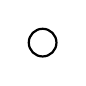
\begin{tikzpicture}[node distance={5mm}, thick, main/.style = {draw, circle, minimum size=1em}] 
	% Sommets :
	\node[main] (0) {}; 
	% Arêtes
	\end{tikzpicture} 
\end{center}
\end{minipage}
\begin{minipage}{0.2\textwidth}
\begin{center}
	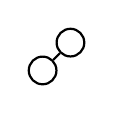
\begin{tikzpicture}[node distance={5mm}, thick, main/.style = {draw, circle, minimum size=1em}] 
	% Sommets :
	\node[main] (0) {}; 
	\node[main] (1) [below left of=0] {};
	% Arêtes
	\draw (0) -- (1);
	\end{tikzpicture} 
\end{center}
\end{minipage}
\begin{minipage}{0.2\textwidth}
\begin{center}
	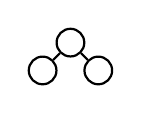
\begin{tikzpicture}[node distance={5mm}, thick, main/.style = {draw, circle, minimum size=1em}] 
	% Sommets :
	\node[main] (0) {}; 
	\node[main] (1) [below left of=0] {};
	\node[main] (2) [below right of=0] {};
	% Arêtes
	\draw (0) -- (1);
	\draw (0) -- (2);
	\end{tikzpicture} 
\end{center}
\end{minipage}
\begin{minipage}{0.2\textwidth}
\begin{center}
	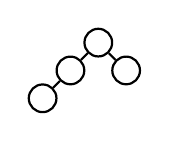
\begin{tikzpicture}[node distance={5mm}, thick, main/.style = {draw, circle, minimum size=1em}] 
	% Sommets :
	\node[main] (0) {}; 
	\node[main] (1) [below left of=0] {};
	\node[main] (2) [below right of=0] {};
	\node[main] (3) [below left of=1] {};
	% Arêtes
	\draw (0) -- (1);
	\draw (0) -- (2);
	\draw (1) -- (3);
	\end{tikzpicture} 
\end{center}
\end{minipage}
\begin{minipage}{0.2\textwidth}
\begin{center}
	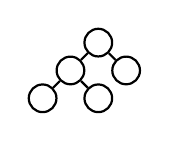
\begin{tikzpicture}[node distance={5mm}, thick, main/.style = {draw, circle, minimum size=1em}] 
	% Sommets :
	\node[main] (0) {}; 
	\node[main] (1) [below left of=0] {};
	\node[main] (2) [below right of=0] {};
	\node[main] (3) [below left of=1] {};
	\node[main] (4) [below right of=1] {};
	% Arêtes
	\draw (0) -- (1);
	\draw (0) -- (2);
	\draw (1) -- (3);
	\draw (1) -- (4);
	\end{tikzpicture} 
\end{center}
\end{minipage}

\begin{minipage}{0.25\textwidth}
\begin{center}
	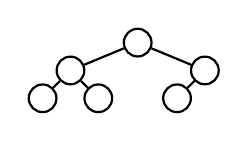
\begin{tikzpicture}[node distance={5mm}, thick, main/.style = {draw, circle, minimum size=1em}] 
	% Sommets :
	\node[main] (0) {}; 
	\node[main] (1) [below left of=0, xshift=-5mm] {};
	\node[main] (2) [below right of=0, xshift=5mm] {};
	\node[main] (3) [below left of=1] {};
	\node[main] (4) [below right of=1] {};
	\node[main] (5) [below left of=2] {};
	% Arêtes
	\draw (0) -- (1);
	\draw (0) -- (2);
	\draw (1) -- (3);
	\draw (1) -- (4);
	\draw (2) -- (5);
	\end{tikzpicture} 
\end{center}
\end{minipage}
\begin{minipage}{0.25\textwidth}
\begin{center}
	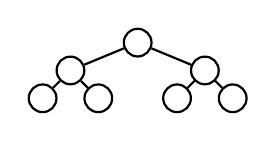
\begin{tikzpicture}[node distance={5mm}, thick, main/.style = {draw, circle, minimum size=1em}] 
	% Sommets :
	\node[main] (0) {}; 
	\node[main] (1) [below left of=0, xshift=-5mm] {};
	\node[main] (2) [below right of=0, xshift=5mm] {};
	\node[main] (3) [below left of=1] {};
	\node[main] (4) [below right of=1] {};
	\node[main] (5) [below left of=2] {};
	\node[main] (6) [below right of=2] {};
	% Arêtes
	\draw (0) -- (1);
	\draw (0) -- (2);
	\draw (1) -- (3);
	\draw (1) -- (4);
	\draw (2) -- (5);
	\draw (2) -- (6);
	\end{tikzpicture} 
\end{center}
\end{minipage}
\begin{minipage}{0.25\textwidth}
\begin{center}
	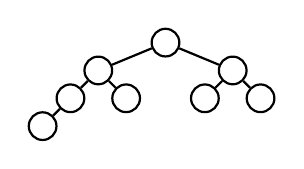
\begin{tikzpicture}[node distance={5mm}, thick, main/.style = {draw, circle, minimum size=1em}] 
	% Sommets :
	\node[main] (0) {}; 
	\node[main] (1) [below left of=0, xshift=-5mm] {};
	\node[main] (2) [below right of=0, xshift=5mm] {};
	\node[main] (3) [below left of=1] {};
	\node[main] (4) [below right of=1] {};
	\node[main] (5) [below left of=2] {};
	\node[main] (6) [below right of=2] {};
	\node[main] (7) [below left of=3] {};
	% Arêtes
	\draw (0) -- (1);
	\draw (0) -- (2);
	\draw (1) -- (3);
	\draw (1) -- (4);
	\draw (2) -- (5);
	\draw (2) -- (6);
	\draw (3) -- (7);
	\end{tikzpicture} 
\end{center}
\end{minipage}
\begin{minipage}{0.25\textwidth}
\begin{center}
	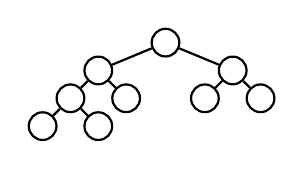
\begin{tikzpicture}[node distance={5mm}, thick, main/.style = {draw, circle, minimum size=1em}] 
	% Sommets :
	\node[main] (0) {}; 
	\node[main] (1) [below left of=0, xshift=-5mm] {};
	\node[main] (2) [below right of=0, xshift=5mm] {};
	\node[main] (3) [below left of=1] {};
	\node[main] (4) [below right of=1] {};
	\node[main] (5) [below left of=2] {};
	\node[main] (6) [below right of=2] {};
	\node[main] (7) [below left of=3] {};
	\node[main] (8) [below right of=3] {};
	% Arêtes
	\draw (0) -- (1);
	\draw (0) -- (2);
	\draw (1) -- (3);
	\draw (1) -- (4);
	\draw (2) -- (5);
	\draw (2) -- (6);
	\draw (3) -- (7);
	\draw (3) -- (8);
	\end{tikzpicture} 
\end{center}
\end{minipage}
\begin{center}
\captionof{figure}{les 9 premiers arbres presque complets\label{fig:arbres_presque_complets}}
\end{center}
\subsubsection{Implantation par tableau}
On observe qu'un arbre presque complet à $n$ étages possède $n-1$ étages complets et $1$ étage remplit à partir de la gauche.

On peut compter le nombre de noeuds par étages :
\begin{itemize}
	\item l'étage $0$ a $2^0$ noeuds
	\item l'étage $1$ a $2^1$ noeuds
	\item \dots
	\item l'étage $0\leq i < n-1$ a $2^{i}$ noeuds
	\item \dots
\end{itemize}
On veut faire correspondre à chacun des noeuds $\{2^{i}-1, \dots, 2^{i+1}-2\}$ d'un étage ses deux sous-arbres gauche et droit. C'est-à-dire qu'on veut trouver une correspondance \textit{injective}\footnote{Une correspondance est une application à valeur dans un produit cartésien (i.e ``une application qui renvoie plusieurs valeurs'')} de $\{2^{i}-1, \dots, 2^{i+1}-2\}$ dans $\{2^{i+1}-1, \dots, 2^{i+2} - 2\}\times \{2^{i+1}-1, \dots, 2^{i+2} - 2\}$\newline
On remarque que :
$$\begin{array}{lclcl}
c & : &\{2^{i}-1, \dots, 2^{i+1}-2\} &\rightarrow &\{2^{i+1}-1, \dots, 2^{i+2} - 2\}^2 \\
  &   & n &\mapsto &(2n+1, 2n+2)
  \end{array}
$$
est une telle correspondance. Elle est représenté par le schéma suivant :

\begin{minipage}{\textwidth}
\begin{center}
\includesvg[width=\textwidth]{tas}
\captionof{figure}{Représentation par tableau d'un arbre presque complet}
\end{center}
\end{minipage}

Comme les noeuds sont numérotés de gauche à droite, si la fin du tableau ne remplit pas un étage, c'est toujours un sous-arbre gauche qui est plus haut qu'un sous-arbre droit. Il s'agit donc bien d'un arbre presque complet.

\begin{minted}[linenos=false]{c}
typedef struct AlmostCompleteTree {
	// Éléments :
	Element *array;
	// nombre d'éléments
	unsigned int size;
	// taille total du tableau (i.e. nb max d'éléments avant redimensionnement) :
	unsigned int capacity; 
} ACT;
\end{minted}
\subsection{Tas minimum}
On décrit ici une implantation efficace des files de priorité grâce à la structure de donnée de \textit{Tas minimum}.

\definition{Arbre tournoi} {
	L'ensemble $A^t_X$ des \textit{arbres tournois} sur un ensemble ordonné $(X, \leq)$ est défini par induction par :
	$$\left\{\begin{array}{cll}
	\mathcal{B} & : & E\in A^t_X \\
	\mathcal{I} & : & \forall g, d\in A^t_X, \forall x\in X, \left[(\forall{n_{l}\in{elts(g)}}, x \leq n_{l}) \wedge (\forall{n_{r}}\in{elts(d)}, x \leq n_r)\right] \Rightarrow (g, x, d)\in A^t_X
\end{array}\right.$$
	En français : la racine d'un arbre tournoi est plus petite que tous les éléments des sous-arbres gauche et droit.
}
\textbf{Exemple :} avec $X = \mathbb{Z}$
\begin{center}
	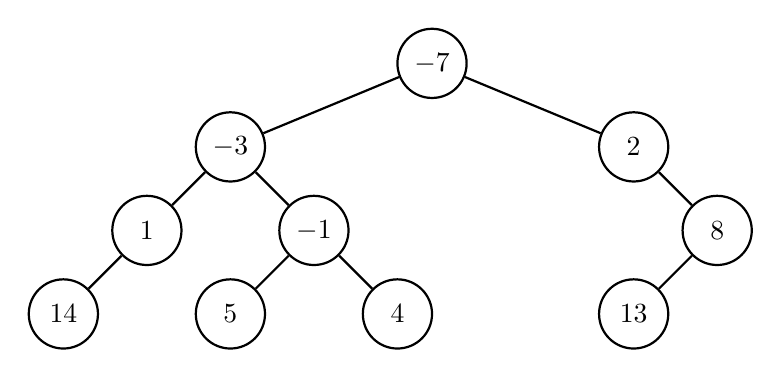
\begin{tikzpicture}[node distance={15mm}, thick, main/.style = {draw, circle, minimum size=2.5em}] 
	% Sommets :
	\node[main] (0) {$-7$}; 
	\node[main] (1) [below left of=0, xshift=-15mm] {$-3$};
	\node[main] (2) [below right of=0, xshift=15mm] {$2$};
	\node[main] (3) [below left of=1] {$1$};
	\node[main] (4) [below right of=1] {$-1$};
	\node[main] (5) [below left of=4] {$5$};
	\node[main] (7) [below right of=4] {$4$};
	\node[main] (6) [below right of=2] {$8$};
	\node[main] (8) [below left of=6] {$13$};
	\node[main] (9) [below left of=3] {$14$};
	% Arêtes
	\draw (0) -- (1);
	\draw (0) -- (2);
	\draw (1) -- (3);
	\draw (1) -- (4);
	\draw (4) -- (5);
	\draw (2) -- (6);
	\draw (7) -- (4);
	\draw (8) -- (6);
	\draw (9) -- (3);
	\end{tikzpicture} 
	\captionof{figure}{Un arbre tournoi\label{fig:abre_tournoi}}
\end{center}
\proposition{Croissance des chemins descendants} Un arbre binaire est un arbre tournoi \textit{si et seulement si} tous les chemins de la racine aux feuilles sont croissants selon les valeurs des noeuds.

\textbf{Démonstration :} par induction, découle immédiatement de la définition

\definition{Tas} {
	Un \textit{tas} est un arbre de tournoi presque complet.
}
\textbf{Exemple :}
\begin{center}
	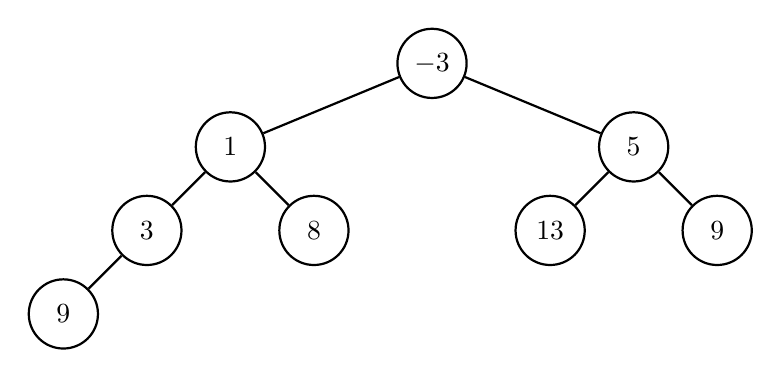
\begin{tikzpicture}[node distance={15mm}, thick, main/.style = {draw, circle, minimum size=2.5em}] 
	% Sommets :
	\node[main] (0) {$-3$}; 
	\node[main] (1) [below left of=0, xshift=-15mm] {$1$};
	\node[main] (2) [below right of=0, xshift=15mm] {$5$};
	\node[main] (3) [below left of=1] {$3$};
	\node[main] (4) [below right of=1] {$8$};
	\node[main] (5) [below left of=2] {$13$};
	\node[main] (6) [below right of=2] {$9$};
	\node[main] (7) [below left of=3] {$9$};
	% Arêtes
	\draw (0) -- (1);
	\draw (0) -- (2);
	\draw (1) -- (3);
	\draw (1) -- (4);
	\draw (2) -- (5);
	\draw (2) -- (6);
	\draw (3) -- (7);
	\end{tikzpicture}
	\captionof{figure}{Un tas minimum\label{fig:tas_min}} 
\end{center}
On peut donc représenter un tas par arbre presque complet, lui-même représenté par un tableau :
\begin{minted}[linenos=false]{c}
typedef ACT Heap;
\end{minted}
Il faut simplement s'assurer lors de l'insertion ou la suppression d'éléments de conserver la structure d'arbre tournoi.
\subsection{Mutateurs}
On décrit dans cette sous-section les deux opérations d'insertion et de suppression dans un tas. En effet, il faut préciser la manière de conserver la structure de tas, donc à la fois d'arbre presque complet mais aussi et surtout de tournoi.

\textbf{Opérations de tamisage :} On désigne par  :
\begin{itemize}
	\item \textit{tamisage bas} l'opération qui consiste à faire \textit{descendre} un élément dans un tas jusqu'à ce qu'il soit plus grand que son élément parent dans l'arbre et plus petit que les éléments de ses sous-arbres gauche et droit
	\item \textit{tamisage haut} l'opération qui consiste à faire \textit{monter} un élément dans un tas jusqu'à ce qu'il soit plus grand que son élément parent dans l'arbre et plus petit que les éléments de ses sous-arbres gauche et droit
\end{itemize}
La descente et la montée se font par échanges successifs d'éléments.
\subsubsection{Insertion}
L'opération est assez simple : on ajoute un élément à la fin du tableau et par tamisage haut on conserve une structure de tas :
\begin{minted}{c}
Heap heap_insert(Heap h, int x) {
	h.size++;
	h.array[h.size - 1] = x;
	heap_top_sieve(h, h.size - 1); // tamisage haut de l'élément d'indice 'h.size - 1' = dernier
	if (h.size >= h.capacity) {
		Element *new = malloc(sizeof(Element) * (h.capacity << 1));
		for (unsigned int i = 0; i < h.capacity; i++) {
			new[i] = h.array[i];
		}
		free(h.array);
		h.array = new;
		h.capacity = h.capacity << 1;
	}
	return h;
}
\end{minted}
\subsubsection{Suppression du minimum}
Si on supprime simplement la racine du tas, ce n'est plus tas. Il faut donc remplacer la racine par un nouvel élément. Il faudrait alors choisir entre la racine du sous-arbre droit ou du sous-arbre gauche, etc\dots Il s'agit en quelque sorte d'un tamisage bas d'un \textit{trou}. C'est étrange.

Le plus simple reste d'échanger la racine du tas avec le dernier élément du tableau, et d'effectuer un tamisage bas sur cette nouvelle racine :
\begin{minted}[linenos=false]{c}
Heap arrayheap_pop_min(Heap h) {
	Element x = h.array[0];
	array_switch(h.array, 0, h.size - 1); // échange avec ou sans effet de bord
	h.size--; // supprimer l'élément
	heap_bottom_sieve(h, 0); // tamisage bas de l'élémeent d'indice '0'
	return x;
}
\end{minted}
\subsection{Exercices}
\exercise{Tamisages}{23} On considère des tas d'entiers dans la suite.
\begin{enumerate}
	\item Écrire une procédure \mintinline{c}{void heap_top_sieve(int *heap, int i);} qui effectue un tamisage haut de l'élément d'indice $i$ dans un tas
	\item Écrire une procédure \mintinline{c}{void heap_bottom_sieve(int *heap, int i);} qui effectue un tamisage bas de l'élément d'indice $i$ dans un tas
	\item Démontrer la correction de chacune des procédures
\end{enumerate}

\exercise{Complexité de la signature}{15} Quelle est la complexité temporelle de chaque routine de manipulation de \textit{FilePriorite} implanté par un tas minimum ? Justifier. En particulier, justifier que le redimensionnement du tableau lors de l'insertion d'éléments n'affecte pas la complexité temporelle amortie de l'insertion, c'est-à-dire que pour tous $n\in\mathbb{N}$, le coût de $n$ insertions dans une file vide est fonction de $O(nlog_2(n))$ dans le pire des cas.

\exercise{Tableau en tas}{} On s'intéresse à la construction d'un tas à partir d'un tableau de $n$ éléments.
\begin{enumerate}
	\item Si on part d'un tas vide et qu'on ajoute un à un par $inserer$ chacun des éléments du tableau, quelle est le coût temporel dans le pire des cas de la construction, selon $n$ ?
	\item Proposer une seconde méthode permettant de construire un tas à partir des éléments d'un tableau dont le coût temporel dans le pire cas soit fonction de $O(n)$
\end{enumerate}

\exercise{Tri par tas}{12}Proposer et implanter en C un algorithme de tri de tableaux qui utilise un tas et dont la complexité temporelle est dans le pire cas fonction de $O(n.log_2(n))$, où $n$ désigne la longueur du tableau en entrée.
\end{document}